\section{Convolutional Neural Networks}
\label{sec:intro}

%-------------------------------------------------------------------------
\subsection{CNN architecture}
Our default CNN architecture is as below: 
\begin{itemize}
	\item 4 convolutional layers with ReLU and Maxpooling
	\item 4 fully connected layers with drop-out and ReLU
	\item Residual connections to every one layers
	\item Use CrossEntropy as a loss function for optimization
	\item The size of convolutional filter size 3
\end{itemize}
In addition, the input of our CNN is resized to 128*128 since Caltech101 dataset has image sizes 100 to 300. Detailed architecture including the dimension of channels are in \cref{fig:cnn_arch}. We tried to choose simple and high-performance model.
\begin{figure}[htbp]
	\centering
	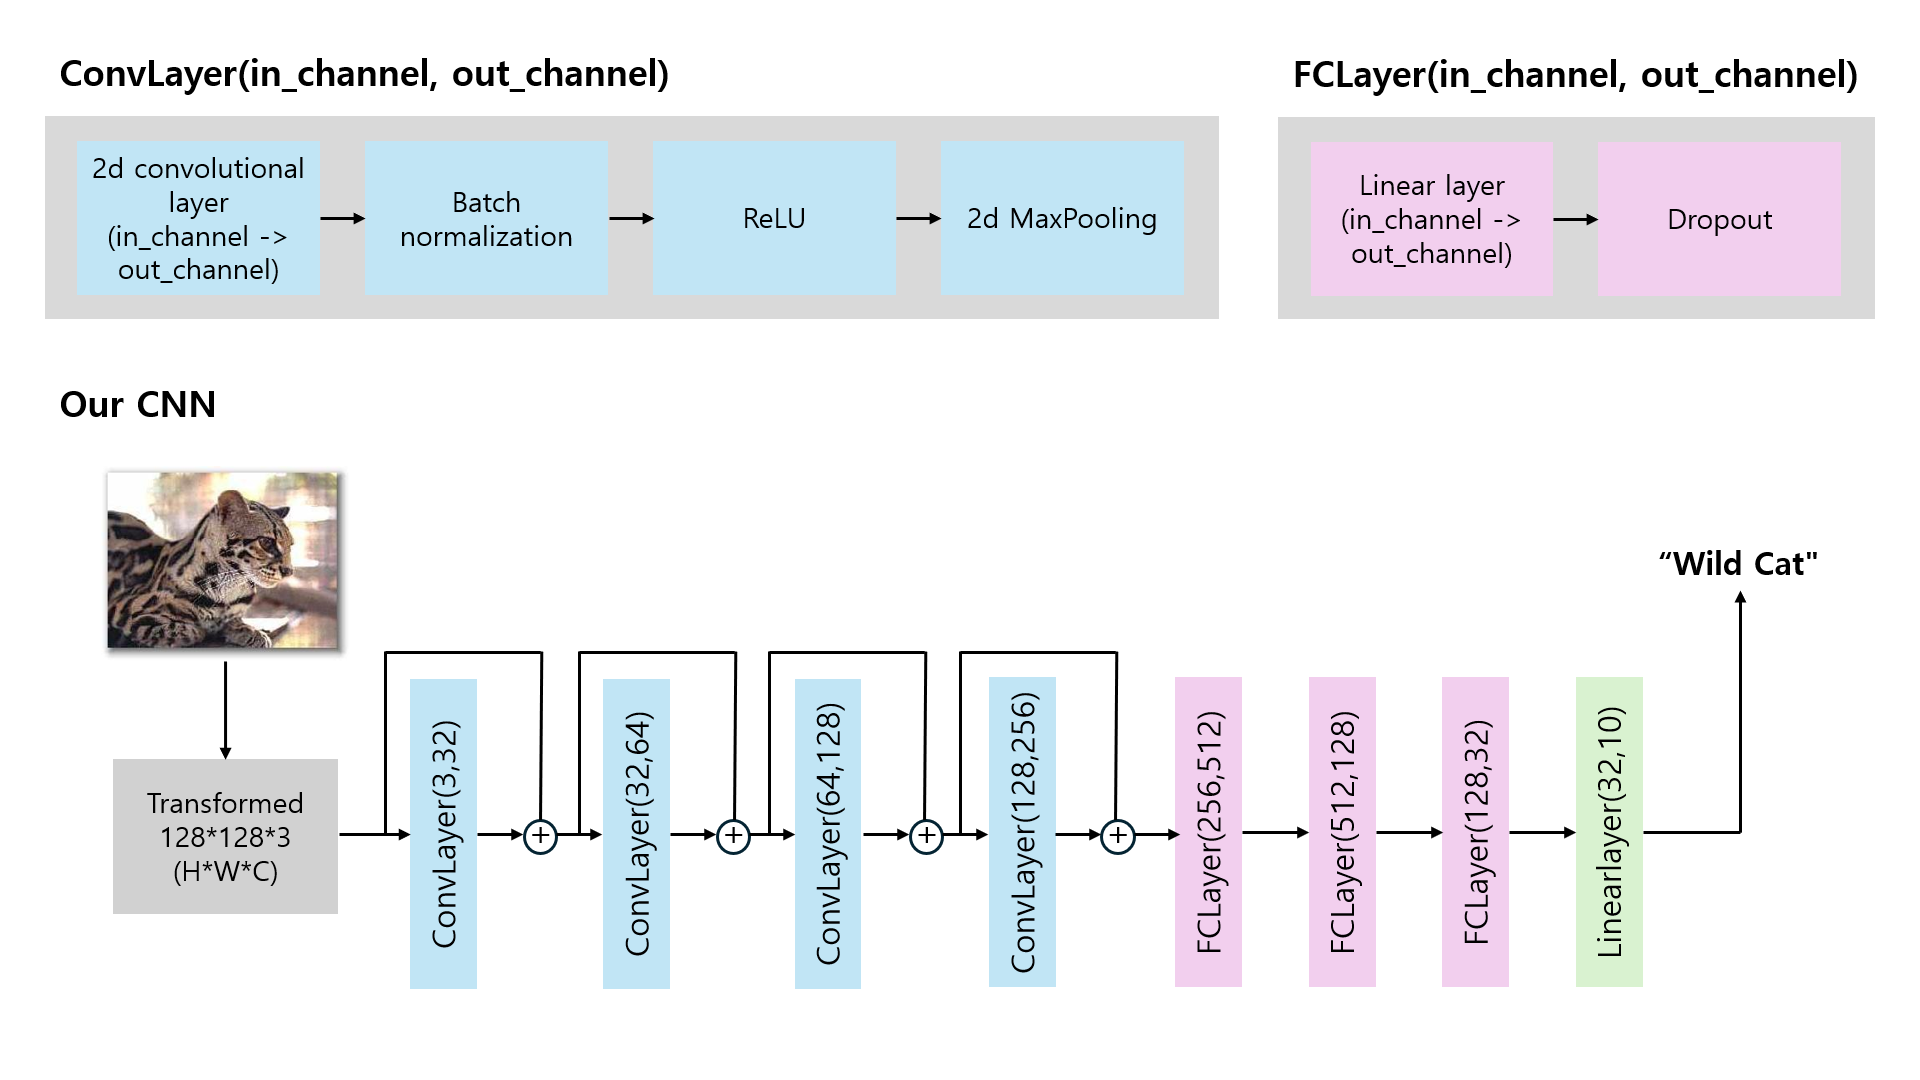
\includegraphics[width=0.7\linewidth]{image/q4-1-arch.png}
	\caption{Our CNN architecture}
	\label{fig:cnn_arch}
\end{figure}

\subsection{Changing architecture}
We changed the number of layers from 3 to 5. As shown in \cref{fig:q4-2-layers}, the test accuracy is highest with 4 layers. When CNN has 3 layers, it is not enough to extract useful features from images. Also when it has 5, we expected over-fitting due to the gradient vanishing. Hence, we selected 4 layers would be the best choice for performance.

Next, we changed the size of kernel to 3, 5, and 7. As \cref{fig:q4-2-kernel} shows, the accuracy is highest when the kernel size is 3 and it decreases afterwards. When the kernel size is small, it is adequate to capture the details of images and when the size is big, it is good to perceive the global scene. However, as our image has 128*128 size, which is small, kernel size 3 is enough to extract useful feature of the image since we also used residual connections. Other sizes might be too big to recognize the detailed features.

Finally, we investigate the effect of residual connections between layers. There are three cases: no connections, connections between every two layers, and connections between each layer. With 4 layers in total, the number of connections are 0, 2, and 4, respectively. The test accuracy, shown in \cref{fig:q4-2-connection}, increases with the number of connections. This improvement is due to the residual connections, which prevent information loss from the initial layers, allowing the CNN to learn more various hierarchical features of the images and their labels.

\begin{figure}[htbp]
	\centering
	\begin{subfigure}[t]{0.3\linewidth}
		\centering
		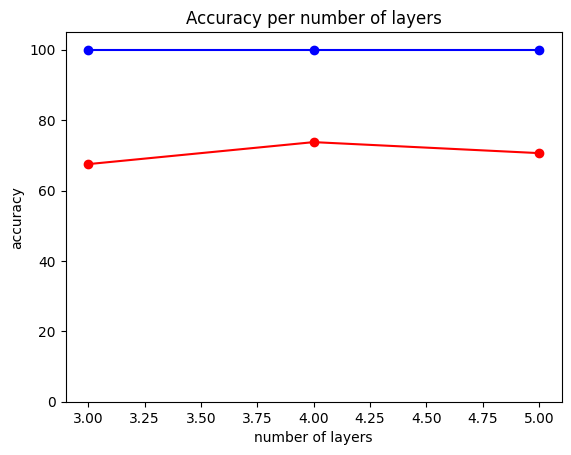
\includegraphics[width=\linewidth]{image/q4-2-layers.png}
		\caption{Accuracy according to layers}
		\label{fig:q4-2-layers}
	\end{subfigure}	
    \hfill
	\begin{subfigure}[t]{0.3\linewidth}
		\centering
		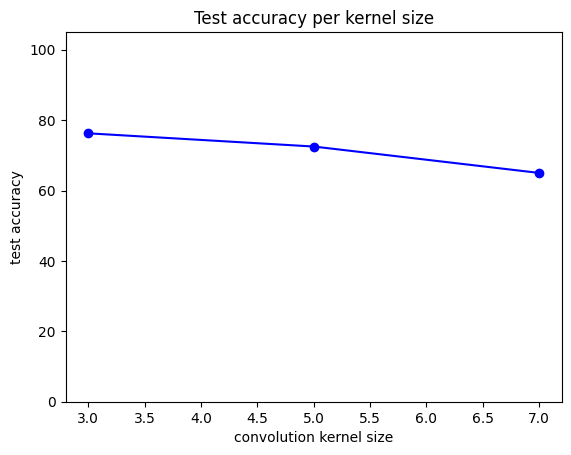
\includegraphics[width=\linewidth]{image/q4-2-kernel.png}
		\caption{Accuracy according to kernel size}
		\label{fig:q4-2-kernel}
	\end{subfigure}%
    \hfill
	\begin{subfigure}[t]{0.3\linewidth}
		\centering
		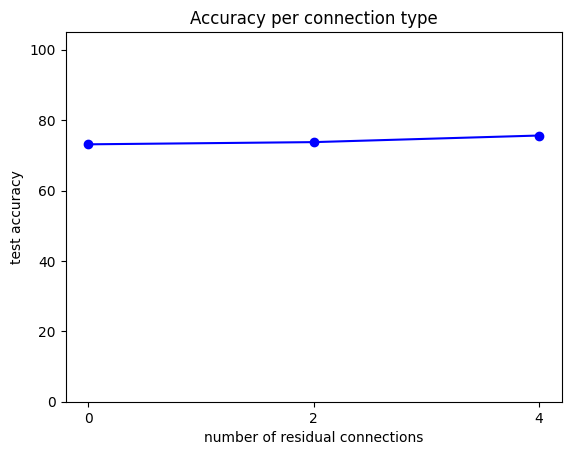
\includegraphics[width=\linewidth]{image/q4-2-connection.png}
		\caption{Accuracy according to connections}
		\label{fig:q4-2-connection}
	\end{subfigure}

	\caption{impact of changing architecture of CNNs}
	\label{fig:cnn_architecture}
\end{figure}

\subsection{Layer normalization}
To explore the effect of the layer normalization method, we tested our model using 4 different methods: batch, layer, instance, and group normalization.

The accuracies according to the batch number for each method are shown in \cref{fig:normalization}. We can check that batch normalization is greatly affected by the size of batch, while the others show consistent accuracy w.r.t. the size of the batch.

For batch normalization, the larger the batch size, the higher the accuracy. This is because larger batches can closely estimate the true distribution of the training data. However, too large batch can reduce accuracy due to the lack of generalization, as batch training sometimes introduces randomness. This is why a batch size of 16 yields the highest accuracy.

In image classification, it is important to catch the difference between feature distribution of within and between classes. Using batch normalization, we can consider class distribution since the normalization is performed on a batch basis. However, other methods only do normalization within a single image, the information related to class statistics is weakened. Hence, their accuracy becomes lower than using batch normalization.

\begin{figure}
	\centering
	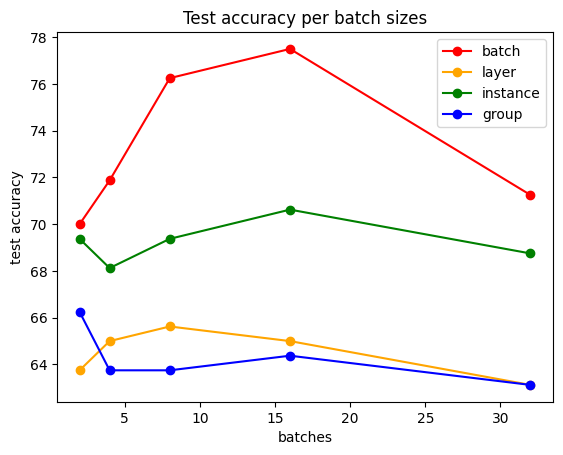
\includegraphics[width=0.4\linewidth]{image/q4-3.png}
	\caption{Accuracy according to normalization types}
	\label{fig:normalization}
\end{figure}

\subsection{Generalization}
In this section, we are going to check the impact of drop-out and L2-regularization term(which is in Deep\_Learning\_intro Lecture Note pg.84). We tested our basic model which has drop-out, the model without drop-out, and the model with L2-regularization on weights. Results are shown in \cref{table:generalization}. The model without generalization method has the lowest accuracy and the model with L2-regularization has the highest accuracy. This is because, dropout randomly deactivate some neurons, so it helps model to avoid overfitting and be good at generalization. And L2-regularization helps model to avoid overfitting by regulate the size of weights.

\begin{table}
	\centering
	\setlength{\tabcolsep}{6pt}
	\renewcommand{\arraystretch}{1.5}
	\resizebox{0.5\linewidth}{!}{
		\begin{tabular}{|c||c|}
		\hline
		& accuracy  \\ \hline\hline
		original & 75.625  \\ \hline
		without dropout & 68.125  \\ \hline
		with L2-regularization term & 76.250  \\ \hline
		\end{tabular}
	}
    \caption{Impact of generalization}
	\label{table:generalization}
\end{table}
	

\subsection{Loss function}
We used CrossEntropy, based on the softmax function, as the default loss function. In this section, we compare it with the SquaredHinge loss. Using CrossEntropy, we achieved 73.75\% accuracy, while SquaredHinge gave a higher accuracy of 80.00\%. This improvement is due to the fact that CrossEntropy relies on probability distribution, while SquaredHinge focuses on the margin between predicted and true classes. Given the small size of our dataset (10 classes), estimating an accurate probability distribution is challenging due to the law of large numbers. Thus, SquaredHinge, which directly considers class margins, performs better. Nevertheless, we utilized CrossEntropy as the default option due to its widespread use.


\subsection{Compressing CNN}
We conduct an experiment on compressing CNN layers using truncated SVD. Our model has 4 fully connected layers with ranks 512, 128, 32, and 10, and we compress the first two layers by 100\% (original), 75\%, 50\%, and 25\% because the last two layers are too small to compress. The result is shown in \cref{fig:cnn_svd}. As expected, a tradeoff between accuracy and efficiency is observed, since compressing the weight matrices improve both time and space-wise efficiency but generate information loss.

\begin{figure}
	\centering
	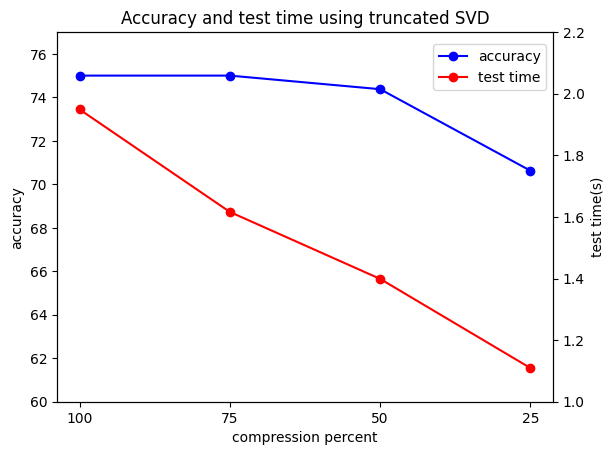
\includegraphics[width=0.4\linewidth]{image/q4-6-svd.png}
	\caption{Accuracy and test time using truncated SVD}
	\label{fig:cnn_svd}
\end{figure}

\subsection{Changing parameters}
We observe the effect of 3 main hyperparameters: learning rate, batch size, and the number of epochs.

\cref{fig:q4-7-lr-train} and \cref{fig:q4-7-lr} show the results of varying the learning rate. We experimented with learning rates of 0.00001, 0.0001, 0.0005, and 0.005. When the learning rate is 0.00001, the model does not reach the local minima, as it is converges very slow. For learning rates of 0.0005 and 0.001, the model oscillates excessively before converging, with the amplitude of oscillation being larger at 0.001 than at 0.0005. This happens because the step size is too large, causing the model to overshoot the local minimum. Therefore, we determined that a learning rate of 0.0001 is optimal for our model. Also, the highest accuracy is achieved at a learning rate of 0.0001, while smaller or larger learning rates result in lower accuracy. 

We trained our model with batch sizes ranging from $2^1$ to $2^6$ and achieved the highest accuracy with a batch size of 16 as in \cref{fig:q4-7-batch}. With small batch sizes, the model learns feature distributions from a limited amount of data, leading to noisy gradient and less smooth converging. However, such noise can allow the model to explore the loss landscape more broadly, helping generalization. This might help the optimizer avoid getting stuck in local minima or saddle points. Therefore, our optimal batch size was 16 because of such tradeoff. Additionally, smaller batch sizes reduce training time due to parallel computing on GPUs.

For the number of epochs, results are shown in \cref{fig:q4-7-epoch}. The accuracy is the highest with 100 epochs because when the number of epoch is not enough, it can cause under-fitting.

\begin{figure}
	\centering
	\begin{subfigure}{0.23\linewidth}
		\centering
		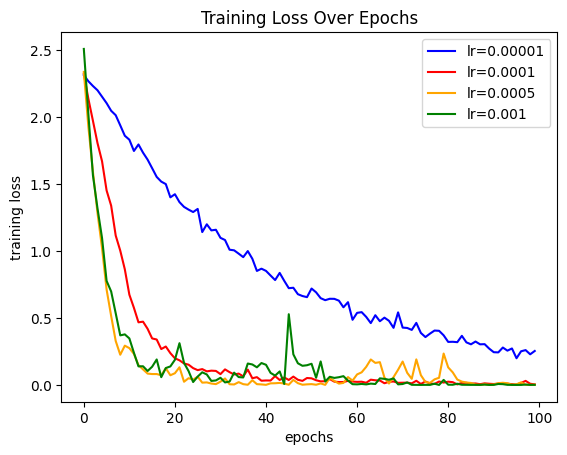
\includegraphics[width=\linewidth]{image/q4-7-lr-train.png}
		\caption{Learning rate training losses}
		\label{fig:q4-7-lr-train}
	\end{subfigure}%
	\hfill
	\begin{subfigure}{0.23\linewidth}
		\centering
		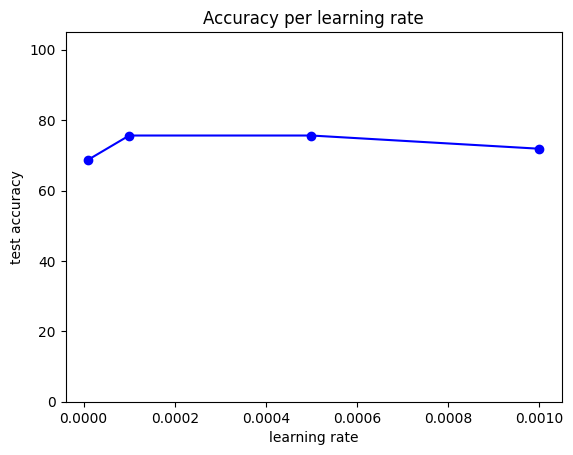
\includegraphics[width=\linewidth]{image/q4-7-lr.png}
		\caption{Learning rate accuracy}
		\label{fig:q4-7-lr}
	\end{subfigure}
	\hfill
	\begin{subfigure}{0.23\linewidth}
		\centering
		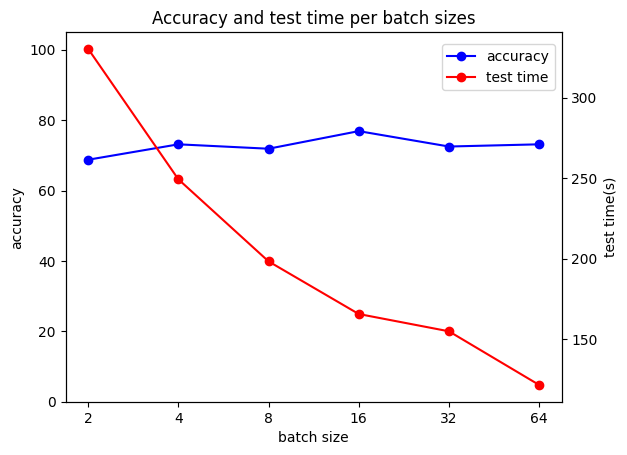
\includegraphics[width=\linewidth]{image/q4-7-batch.png}
		\caption{Batch size accuracy}
		\label{fig:q4-7-batch}
	\end{subfigure}
	\hfill
	\begin{subfigure}{0.23\linewidth}
		\centering
		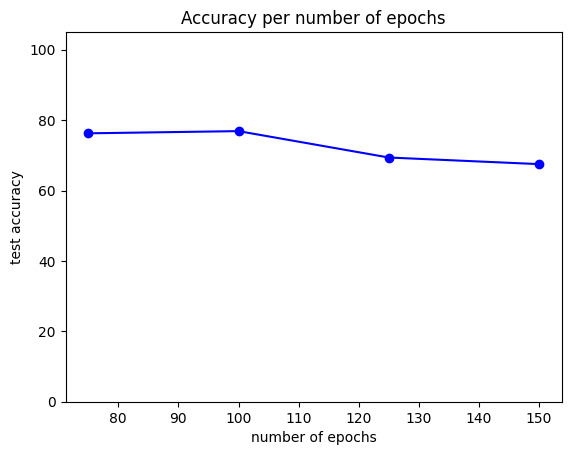
\includegraphics[width=\linewidth]{image/q4-7-epoch.png}
		\caption{Epoch accuracy}
		\label{fig:q4-7-epoch}
	\end{subfigure}
	\caption{Changing hyper-parameters of CNN}
	\label{fig:q2}
\end{figure}

\subsection{Pre-trained model}
We compared two initialization methods: fine-tuning pre-trained weight model and training from random initialization. For this experiment, we used pre-trained ResNetModel(microsoft/resnet-50, trained with ImageNet)\cite{ref1} and fine-tuned it with Caltech101 dataset. Due to our limited computing resource, we only train it with 10 epochs. When we use pre-trained weights and fine-tuned them, we get 99.33\% accuracy while training from scratch represents 21.33\%. Based on this result, the initialization weight highly affects the deep learning's convergence. It is because, since our pre-trained weights are obtained from performing same task(image classification) with large dataset, such initialization weights already have some useful features for image classification. 

\subsection{Comparison with other methods}
Our CNN model's accuracy is about 75\%, which is better than Q2 and Q3 as shown in \cref{table:accuracy}. This is because CNN can do end-to-end learning from feature extraction to classification, unlike Q2 and Q3's model. In other words, k-means or random forest vocabulary followed by random forest classification does not allow end-to-end learning, making it difficult to determine whether the vector quantisation result includes beneficial features for classification. However, CNN can automatically learn various meaningful representations directly from raw data.

\begin{table}[htbp]
	\centering
	\setlength{\tabcolsep}{6pt} % Adjust column spacing
	\renewcommand{\arraystretch}{1.5} % Adjust row height
	\resizebox{0.5\textwidth}{!}{ % Scale table to fit text width
		\begin{tabular}{|c||c|c|}
			\hline
			& Train Accuracy (\%) & Test Accuracy (\%) \\ \hline\hline\
			K-means Codebook - RF Classifier & 99.50 & 68.5   \\ \hline
			RF Codebook - RF Classifier & 97.80 & 60.67  \\ \hline
			CNN & 100.00 & 75.625  \\ \hline
		\end{tabular}
	}
	\caption{Accuracy of Models}
	\label{table:accuracy}
\end{table}